\section{项目部署与交付}

本章说明项目如何从本地算法实现变成可打开、可运行、可复现的量子信息基础大作业成果。交付
形态包括公开仓库、在线前端、服务器接口、协议工具、命令行、测试验证和报告 PDF。
这些材料共同支撑网页体验、接口调用和本地复现实验。

\subsection{项目组织}

公开仓库是项目总览。仓库首页说明项目目标、安装方式、在线演示、服务接口、命令行
用法、样例线路、拓扑选择和主要实验结果。报告 PDF、网页演示、示例线路、测试脚本
和说明文档都放在同一仓库中，避免出现“报告写了一套、代码在另一套环境中”的问题。

项目组织遵循量子信息基础大作业的交付逻辑：仓库说明项目目标和运行方式，在线前端呈现交互
效果，命令行和服务接口支持复现实验，公开测试维持说明、接口和示例的一致性。这个
结构把算法、系统和实验联系在一起。

图 \ref{fig:github-entry} 展示公开仓库入口。仓库首页把 README、许可证、目录结构、
在线前端和提交历史放在同一视图中，读者进入仓库后可以先阅读快速入口，再根据需要
打开网页、启动服务或运行本地测试。

\begin{figure}[H]
  \centering
  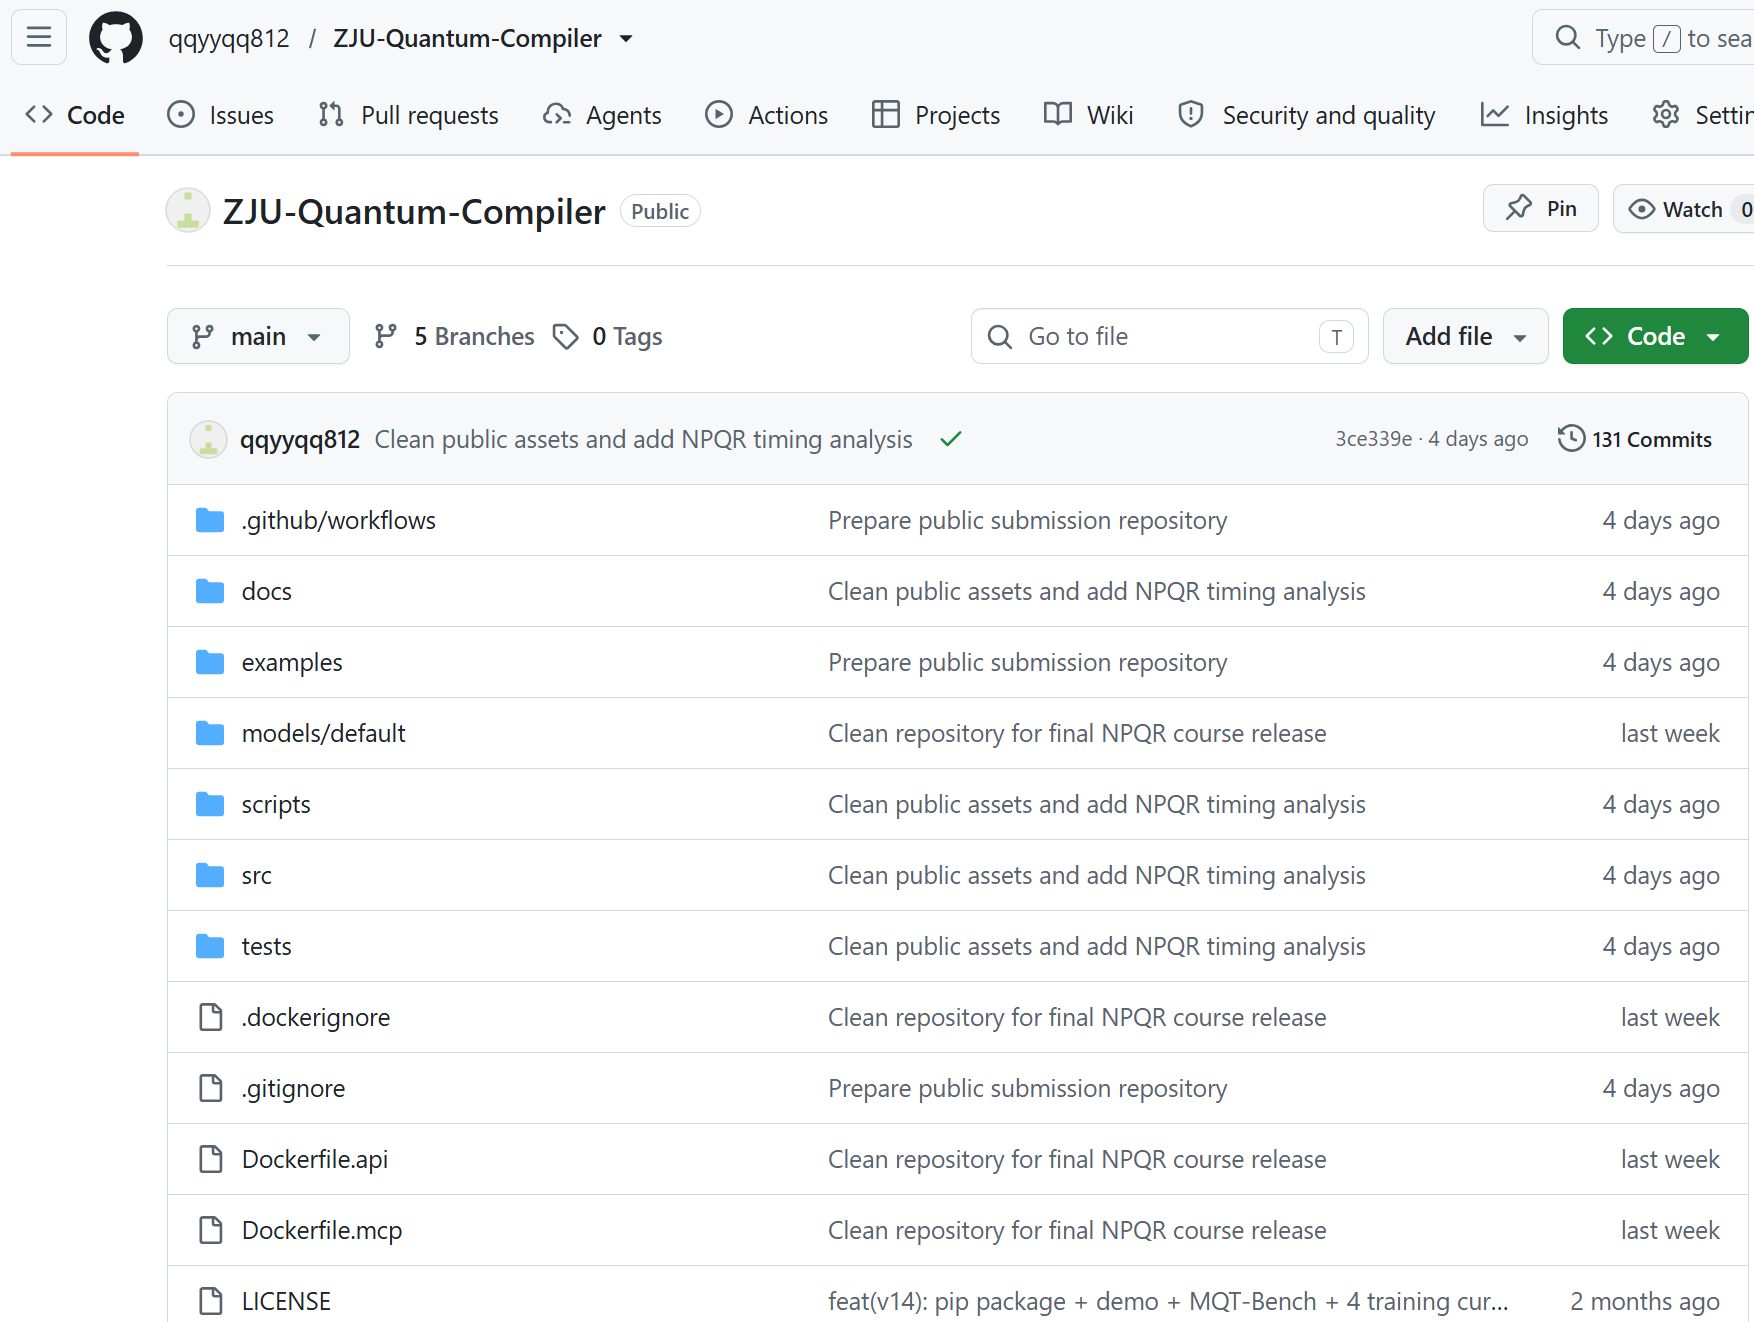
\includegraphics[width=0.92\linewidth]{figures/github-entry.png}
  \caption{仓库入口}
  \label{fig:github-entry}
\end{figure}

图 \ref{fig:project-timeline} 展示项目周期。整体工作先完成 SABRE 基线与最小路由
闭环，再围绕 NPQR 增加初始映射、模型评分、束搜索、修复和复放；随后把算法封装为
网页、REST、MCP 和命令行；最后整理公开仓库、在线前端、服务器服务、测试验证和
报告材料。

\begin{figure}[H]
  \centering
  \begin{tikzpicture}[
  node distance=0.45cm,
  stage/.style={
    rectangle,
    draw=blue!45!black,
    fill=blue!4,
    rounded corners=2pt,
    text width=0.18\linewidth,
    align=left,
    inner sep=5pt,
    font=\footnotesize
  },
  arrow/.style={-{Latex[length=2.2mm]}, thick, draw=blue!45!black}
]
\node[stage] (s1) {
  \textbf{阶段一}\\
  基线闭环\\
  QASM、拓扑、SABRE、最小路由任务
};
\node[stage, right=0.45cm of s1] (s2) {
  \textbf{阶段二}\\
  NPQR 迭代\\
  初始映射、模型评分、束搜索、修复
};
\node[stage, right=0.45cm of s2] (s3) {
  \textbf{阶段三}\\
  系统封装\\
  REST、MCP、CLI、前端控制台
};
\node[stage, right=0.45cm of s3] (s4) {
  \textbf{阶段四}\\
  交付整理\\
  GitHub Pages、华为云、报告与测试
};
\draw[arrow] (s1) -- (s2);
\draw[arrow] (s2) -- (s3);
\draw[arrow] (s3) -- (s4);
\end{tikzpicture}

  \caption{项目周期}
  \label{fig:project-timeline}
\end{figure}

\subsection{在线前端}

前端采用静态网页发布，适合课程展示和跨设备访问。静态页面不要求访问者先配置本地
环境，打开后即可查看示例、拓扑、指标面板和轨迹回放。当服务器接口可达时，页面
会把编译请求发送到后端；当读者只想了解功能时，页面中的样例和说明也能独立展示
项目结构。

GitHub Pages 适合承载这类公开展示页面：它与公开仓库天然绑定，更新流程清晰，访问链接
固定。前端不保存实验结论本身，而是作为编译结果
的展示层；真正的路由、基线比较和轨迹生成仍由共享编译核心完成。

\subsection{服务器部署}

服务器部署负责处理真实编译请求。后端服务接收线路、后端选择和拓扑名称，调用同一
编译核心，并返回路由后线路、指标和轨迹。服务端提供健康状态、样例列表、拓扑查询、
线路校验、同步编译、异步任务和实验摘要等能力。异步任务用于耗时稍长的线路，避免
浏览器在等待过程中失去响应。

云端部署使用容器化方式固定运行环境。这样做有两个优点：一是依赖库、模型文件和
服务启动方式可以被明确记录；二是本地运行和服务器运行使用同一套调用方式，减少“本地
能跑、线上不一致”的问题。报告中的在线前端与服务器接口保持分工：前端负责交互，
服务器负责计算。

\subsection{工具接口}

除普通网页和 REST 调用外，项目还提供 MCP 与命令行两类接口。MCP 面向支持工具调用
的客户端，适合把量子编译能力接入自动化工作流；命令行面向本地复现，用于确认
安装状态、编译内置样例和生成对照矩阵。

这两类接口的价值在于扩展使用场景。网页适合展示，REST 适合应用集成，MCP 适合工具
编排，命令行适合复现实验。四种调用方式共享同一结果字段，因此不会形成互相矛盾的结果
口径。

\subsection{测试与复现}

公开交付包含一组基础测试。测试覆盖服务契约、网页静态契约、
README 内容、部署配置和材料完整性。这里的测试目标不是证明算法在所有可能线路上
最优，而是保证说明、接口和示例能够互相对应。

表 \ref{tab:delivery-checklist} 汇总主要交付项。正文只解释交付结构，具体命令放在
附录中，作为复现实验的命令说明。

\begin{table}[H]
  \centering
  \caption{交付清单}
  \label{tab:delivery-checklist}
  \begin{tabularx}{\linewidth}{lY}
    \toprule
    交付项 & 作用 \\
    \midrule
    公开仓库 & 汇总代码、报告、样例、测试和说明文档。\\
    在线前端 & 展示线路输入、拓扑选择、轨迹回放和指标对比。\\
    服务器接口 & 处理真实编译请求，返回路由线路、指标和轨迹。\\
    MCP 服务 & 为工具客户端提供状态查询、样例读取和编译调用能力。\\
    命令行接口 & 支持本地安装确认、示例编译和对照矩阵生成。\\
    测试验证 & 覆盖公开接口、网页契约、README 和材料完整性。\\
    报告 PDF & 汇总理论基础、SABRE 复现、NPQR 方法、系统部署和实验结果。\\
    \bottomrule
  \end{tabularx}
\end{table}

